% This must be in the first 5 lines to tell arXiv to use pdfLaTeX, which is strongly recommended:
% (In particular, the hyperref package requires pdfLaTeX in order to break URLs across lines.)
\pdfoutput=1
% Define document class:
\documentclass[11pt]{article}
% Drop the "[review]" option to generate the final version:
%\usepackage[review]{acl2021}
%\usepackage{acl2021}
\usepackage{acl2021}
% include images
% (see https://www.overleaf.com/project/6250c0be2e540603fbab4d23)
\usepackage{graphicx} %package to manage images
\graphicspath{ {./images/} }
\usepackage[rightcaption]{sidecap}
\usepackage{wrapfig}
% Double horizontal line in tables
% (see https://tex.stackexchange.com/questions/130818/how-to-draw-a-double-hline-in-a-table-without-interrupting-vertical-lines)
\usepackage{hhline}
% Include standard packages:
\usepackage{times}
\usepackage{latexsym}
% For proper rendering and hyphenation of words containing Latin characters (including in bib files):
\usepackage[T1]{fontenc}
% This assumes UTF8 encoding:
\usepackage[utf8]{inputenc}
% This is not strictly necessary, and may be commented out, but it will improve the layout of the manuscript, and will typically save some space:
\usepackage{microtype}
% If the title and author information does not fit in the area allocated, uncomment the following and set <dim> to 5cm or larger:
%\setlength\titlebox{<dim>}
\title{Final Paper for XCS224U Project \emph{gNER}}
% Author information can be set in various styles:
% (i) a) For several authors from the same institution:
% \author{Author 1 \and ... \and Author n \\
%         Address line \\ ... \\ Address line}
% (i) b) if the names do not fit well on one line use
%         Author 1 \\ {\bf Author 2} \\ ... \\ {\bf Author n} \\
% (ii) For authors from different institutions:
% \author{Author 1 \\ Address line \\  ... \\ Address line
%         \And  ... \And
%         Author n \\ Address line \\ ... \\ Address line}
%  (iii) To start a seperate ``row'' of authors use \AND, as in
% \author{Author 1 \\ Address line \\  ... \\ Address line
%         \AND
%         Author 2 \\ Address line \\ ... \\ Address line \And
%         Author 3 \\ Address line \\ ... \\ Address line}
\author{
	Matthias Droth\\
	matthias.droth@gmail.com
	\And
	Martin Nigsch\\
	martin@nigsch.eu
	\And
	Vasco Ribeiro\\
	vascosousaribeiro@yahoo.com
}

% DOCUMENT START
\begin{document}
\maketitle

% ABSTRACT
\begin{abstract}
In our project gNER, we assess how to efficiently perform Named Entity Recognition (NER) in German language in a real-life scenario with scraped newspaper data. We assess a small range of model choices and to a minor extent annotation choices with the overall goal of finding an optimum between maximizing extraction accuracy while minimizing annotation and computational costs. The data features only little variation in terms of vocabulary and style, yet is relevant in practical life as it contains property prices as sold in the Vorarlberg region in Austria.
\end{abstract}

% Introduction
\section{Introduction}
In this document, we implement and apply a variety of neural-network based models to perform named entity recognition on our custom dataset. We begin by experimenting with linear-chain Conditional Random Fields (CRF) stand-alone and after adding custom feature functions. Next, we experiment with a one-layer LSTM which we then proceed to associate with a CRF layer. 
\newline We hypothesize that CRF algorithms perform on par with deep learning algorithms when trained only on a relatively small named entity recognition (NER) dataset such as the one we are working with. Finding an architecture that produces acceptable results even in the presence of small annotated datasets can be of great value to practitioners looking for high quality out-of-sample inference.
\newline We find that simple CRF models outperform LSTM-based networks. This outperformance is magnified by the application of custom feature functions (such as word capitalization and use of gazetteers).

% Related work
\section{Related work}
We seek to extract named entities out of German text at a minimum overall cost. In order to do so, there are several areas to explore: (i) better models making better use of training data annotation, (ii) pretraining with colloquial vs.~domain specific language, (iii)  model choices beyond the obvious hyperparameter optimization (e.g. tokenization), and (iv) advantageous annotation strategies where the marginal benefit of adding more annotations is the greatest. 

While we acknowledge the potential of cleverly chosen annotation strategies, we think that this area is the most time consuming and the hardest to implement within the time available for this project. For that reason, we focus on comparing NER efficiency resulting from the choice of algorithms as well as their pretraining. 

A large part of our project focusses on CRF and LSTM architectures. We drew heavily on work from \citet{MAL-013} for a theoretical understanding of CRF's. We further deepened this knowledge by working through \href{http://www.cs.columbia.edu/~mcollins/crf.pdf}{course materials} from \href{http://www.cs.columbia.edu/~mcollins/}{Michael Collins} of Columbia University. For joining LSTM and CRF architectures we followed approaches laid out in \citet{DBLP:journals/corr/HuangXY15} and \citet{lample-etal-2016-neural}. In \citet{yadav-bethard-2018-survey} a survey of research in Named Entity Recognition (NER) is performed with a particular emphasis on comparing results achieved by more recent approaches. 

Using well thought-out paper selection criteria, the survey starts with knowledge-based and unsupervised bootstrapped systems moving on to a description of both classic feature-engineered supervised systems as well as modern feature-inferring neural network models. Drilling in on the latter the paper establishes the taxonomy as word-level, character-level and hybrid (character+word and, finally, char+word+affix). The vast majority of architectures presented rely on bi-directional LSTM layers coupled with CRFs for final classification. The paper then proceeds to summarize the results obtained by each type of model on standard NER datasets enabling an overall ranking to be determined (in order of increasing performance) as follows: 1. Feature-engineered systems (least performant even despite using domain-specific rules, knowledge, features and lexicons); 2. Word-based and char-based models; 3. Char+word based hybrid models; 4. Char+word+affix hybrid models. The char+word+affix model showcases the potential of combining useful past insights with modern neural network models which, the paper concludes, represents an exciting avenue for future research.

% Data
\section{Data}

The base data consists of articles from a regional Austrian Newspaper called \href{https://www.vn.at/tags/grund-und-boden}{Vorarlberger Nachrichten}. These articles summarize recent changes in ownership in real estate and cover about a quarter of all property transactions. 

\subsection{Procurement}

In order to be as complete as possible also for future use of the data, we have developed a scraper which logs into the newspaper and fetches a full list of urls which are of interest. In order to avoid fetching an existing url multiple times when refreshing the scraping, each url is assigned a unique ID with the \href{https://www.blake2.net}{blake2b} algorithm. 

In a further step, for every url possible images are extracted and stored, as well as a JSON file containing the HTML and an extraction of just the textual portion of the HTML. The final extract contains 3701 individual scraped newspaper articles published between 2019 and March 2022. 

\subsection{Annotation}

In order to train a NER model, the tool \href{https://prodi.gy/}{Prodigy} has been used to manually annotate. The following eleven entities were annotated for 140 examples, i.e., a fraction of $4\%$ of the full dataset:

\begin{itemize}
    \item ORT (location)
    \item VERKAEUFER (seller)
    \item KAEUFER (buyer)
    \item GESAMTPREIS (total price)
    \item FLAECHE (area)
    \item STRASSE (street)
    \item DATUM\_VERTRAG (date of contract)
    \item DATUM\_VERBUECHERUNG (date of entry in cadastral register)
    \item IMMO\_TYP (type of property)
    \item QMPREIS (price per square meter)
    \item TERRASSENGROESSE (size of terrace)
\end{itemize}

The annotation process itself was sped up by the use of a gazetteer for the towns known in the region of Vorarlberg. Furthermore, a regular expression was used to identify \emph{total price}. 

When annotating, it became apparent that the premeditated annotation scheme isn't necessarily unique: sometimes in real language, the same two words \emph{"private persons"} were used to designate non-identified individuals as buyers and sellers, which made annotation of overlapping entities necessary. Furthermore, in some instances for a house, the square meters of the building were given as well as the square meters of the plot of land. This isn't necessarily a problem for the annotation itself, but it is expected to render making sense of the extracted data much more difficult. 

A need for an annotation strategy was identified, as there are choices to be made, e.g., when annotating a price: whether the currency, "Euro", is part of the price or not shouldn't depend on the annotator, but be consistent across the dataset. 

Similarly, technical difficulties were encountered during annotation as depending on the length of the entity to be annotated, a trailing period (".") was sometimes marked in the user interface. 

\subsection{Postprocessing}

All data extracted out of the prodigy database was written into a single JSON file. 

Given how the user needs to mark an entire token with a cursor in order to assign a label suggested by prodigy, it is very easy for a trailing period to be accidentally included in the marked text. As such we removed last trailing non-alphanumeric characters but only for those tokens that are the last in a chain of (possibly many) tokens classified in same class. In other words, we leave unchanged non-alphanumeric characters that aren't either the last character of a token or that are the last character of a token but that token is itself part of a group of successive tokens all classified in the same label (named entity). For, e.g., we want to change labelling of following tokens related to a corporation "ABC GmbH." so as to only label "ABC GmbH" (i.e. remove the trailing ".").

The 140 instances are split into a training set of 104 fully annotated instances and a test set of 36 fully annotated instances. Evaluation during development relies on three fold cross-validation using the training set. The test set is only used for final evaluation.

\subsection{Summary Statistics}

As is to be expected for a usual NER dataset, the unlabelled class is much more prominent than labelled classes. Indeed, approximately 75\% of all distinct tokens are unlabelled. The lexicon is quite small at 1,152 distinct tokens, with 37\% of these being numbers. Table \ref{datstat} lists further summary statistics of our dataset.

% <table>
\begin{table}[h]
\centering
\caption{Overview of our dataset's statistics. The mean (standard deviation) is denoted by $\mu$ ($\sigma$).}
\label{datstat}
\begin{tabular}{|l|r|}
\hline
Dataset statistic & Value\\
\hhline{|=|=|}
Total sample texts & 140\\
\hline
Total tokens & 7717\\
\hline
Total distinct labels & 1283\\
\hline
Total distinct labelled tokens & 1822\\
\hline
Number of tokens per label: $\mu$ & 1.4\\
\hline
Number of tokens per sample text: $\mu$ & 55\\
\hline
Number of tokens per sample text: $\sigma$ & 23\\
\hline
Number of labels per sample text: $\mu$ & 9\\
\hline
\end{tabular}
\end{table}
% </table>

%\begin{center}
%\begin{tabular}{ |c|c|c| } 
% \hline
% Total Sample Texts & 140 \\
% Total Tokens & 7,717 \\
% Total Distinct Labels & 1,283 \\ 
% Total Distinct Labelled Tokens & 1,822 \\
% Avg. No. of Tokens per Label & 1.4 \\ 
% Avg. No. of Tokens per Sample Text & 55 \\ 
% Std. Dev. No. of Tokens per Sample Text & 23 \\
% Avg. No. of Labels per Sample Text & 9 \\ 
% \hline
%\end{tabular}
%\end{center}

% Models
\section{Models}
We relied substantially on linear-chain CRFs \citep{laffertyCrf, mccallum-li-2003-early, MAL-013}. By explicitly modelling label-word emissions and label-label transitions, these models introduce dependencies between successive classes that are actual features of the NER process. Plain LSTM-based sequence classification models, on the other hand, treat the classification of successive tokens as effectively independent.

For the pytorch-based CRF implementation, we computed starting emissions from conditional probabilities of emission to each word from each one of the 11 class labels. Beyond the default CRF model architecture, we have tried to apply it on top of a bidirectional one-layer LSTM network. We essentially took the outputs from the forward-pass of the LSTM layer as the model (label-word) emission probabilities for the CRF layer on top. We drove the neural-network optimization process on the loss expressed as the negative log likelihood coming from the optimal path as per the Viterbi algorithm \citep{forney1973viterbi}.

% Experiments
\section{Experiments}
As an initial baseline, we use a custom model that always predicts the most common label in the training data. The $F_1$ scores of this and all other models we have implemented are shown in Table \ref{scoresTab}

We then experimented with a standard CRF (using the \href{https://sklearn-crfsuite.readthedocs.io/en/latest/}{sklearn-crf} package). By adding some feature functions such as capitalization and a gazetteer for the location field, we were able to further improve the macro averaged $F_1$ score to 88.6\%.

In terms of metrics we feel macro average $F_1$ score is the most appropriate for an NER use case such as ours that typically has a very large dominant class (the unlabelled or \emph{outside} class). Weighted average $F_1$ scores would not be appropriate as they would be focusing precisely on the one (unlabelled or \emph{outside}) class that we care the least about. By weighting each class equally, the macro average $F_1$ score attributes importance to correct labelling of all classes.

Regarding metrics, a relevant topic is whether for two texts of equal size and relevance, we are indifferent between identifying named entities in one text very well but in the other very poorly versus identifying entities in both texts with similar, average success. In case we decide only 100\% correctness is appropriate then we can rely on a strict $F_1$ measure.

Finally, we want to address the critical importance of loss functions used in the optimization process. As discussed in \citet{li-etal-2020-dice}, the typical optimization process relies on loss functions (e.g. cross-entropy loss) that weigh each observation equally. This is not the ideal approach in particular in the presence of the dataset skew we mentioned earlier.

Turning back to the different model architectures, we have tried to replicate the same CRF model under the \href{https://pytorch-crf.readthedocs.io/en/stable/}{pytorch} paradigm. The intent, here, was not only to explore a different implementation but also to lay the groundwork to add the CRF model to the pytorch-based Stanford XCS224U class  \href{https://github.com/cgpotts/cs224u}{codebase}. As we show below, the results are not entirely encouraging with macro average $F_1$ scores dropping from 66.1\% to 25.2\% for what should essentially be the same CRF model with no feature functions. Further work needs to be done here to account for these differences.

Next, we applied the XCS224U class code RNN Sequence Labeling section in \href{https://github.com/cgpotts/cs224u/blob/master/tutorial_pytorch_models.ipynb}{Tutorial Pytorch Models}. Results here were also considerably underwhelming at 9.0\% macro average $F_1$ score (just above always predicting the most common \emph{outside} class).

We have also used an explicit implementation of the CRF model (including the Viterbi algorithm) and connected it with features coming from an LSTM network. This model produced good results at average $F_1$ of 74.7\%, improving over the base CRF with no feature functions (66.1\%).

Finally, we attempted to implement a (pytorch-based) CRF layer on top of the XCS224U LSTM Sequence Labeler (RNNSequenceLabeler class). Judging from the results (at the level of the simple majority baseline and very different from the LSTM-CRF network mentioned just before) it appears there is still an implementation error, here.

%\begin{center}
%\begin{tabular}{ | m{1cm} | m{5cm}| m{2em} | m{2em} |} 
% \hline
% Model Architecture & M. Avg F1 & Strict F1 \\ [0.5ex] 
% \hline\hline
% 1. Most Common & 7.1 & 0.0\\ 
% \hline
% 2. CRF & 66.1 & 11.1\\
% \hline
% 3. CRF (feature f.) & 88.6 & 30.6  \\
% \hline
% 4. CRF (pytorch) & 25.2 & 0.0  \\
% \hline
% 5. LSTM (XCS224U) & 9.0 & 0.0 \\ 
%  \hline
% 6. LSTM+CRF & 74.7 & 26.5 \\ 
%  \hline
% 7. LSTM+CRF (XCS224U) & 6.9 & 0.0 \\ 
% \hline
%\end{tabular}
%\end{center}

% <table>
\begin{table}[t]
\centering
\caption{Macro-averaged $F_1$ ($F_{1, \overline{\rm{macro}}}$) and strict $F_1$ ($F_{1, \rm{strict}}$) scores (in \%) of different models on our test set.}
\label{scoresTab}
\begin{tabular}{|l|l|l|}
\hline
Model & $F_{1, \overline{\rm{macro}}}$ & $F_{1, \rm{strict}}$\\
\hhline{|=|=|=|}
Most common & $7.1$ & $0.0$\\
\hline
CRF & $66.1$ & $11.1$\\
\hline
CRF (feature functions) & $88.6$ & $30.6$\\
\hline
CRF (pytorch) & $25.2$ & $0.0$\\
\hline
LSTM (xcs224u) & $9.0$ & $0.0$\\
\hline
LSTM+CRF & $74.7$ & $26.5$\\
\hline
LSTM+CRF (xcs224u) & $6.9$ & $0.0$\\
\hline
\end{tabular}
\end{table}
% </table>


% <figure>
\begin{figure}[h!]\centering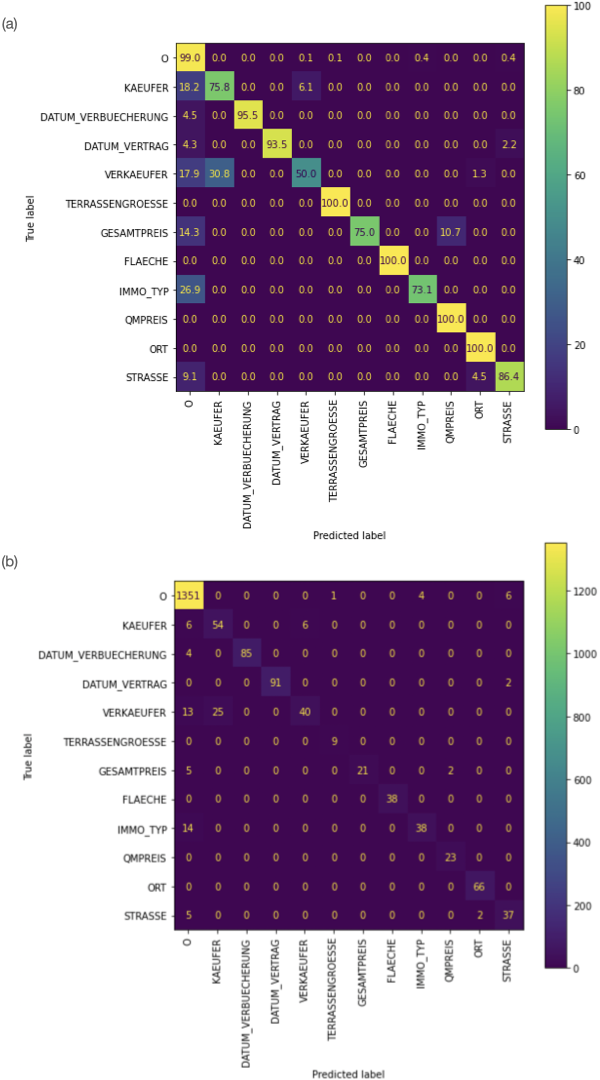
\includegraphics[width=\linewidth]{confMat.png}
\caption{Confusion matrix for the best \emph{CRF (feature function)} model found via hyperparameter search. (a) The cell in row $i$ and column $j$ shows the percentage of instances of the true label (row $i$) that have been predicted as belonging to  the predicted label (column $j$). Disregarding rounding errors, predictions add up to 100\% per true label. (b) The same confusion matrix but with raw counts per cell.}
\label{confMat}
\end{figure}
% </figure>


% Analysis
\section{Analysis}
The macro-averaged $F_1$ scores for our models cover a wide range: from 6.9\% to 88.6\%. The latter, top score indicates that the task of named entity recognition can be performed successfully even with a dataset as small as ours (104 instances for development, 36 instances for final evaluation). Our baseline model achieves a macro-averaged $F_1$ score of 7.1\% by always naively predicting the most common \emph{outside} label, thus indicating an implementation error for the \emph{LSTM+CRF (xcs224u)} model and, to a lesser extent, for the \emph{LSTM (xcs224u)} model. The \emph{CRF (pytorch)} model performs significantly better than our baseline model but further analysis would be required to understand the gap between this and the higher scoring models (\emph{CRF}, \emph{LSTM+CRF}, and \emph{CRF (feature functions)}.

Fig.~\ref{confMat} (a) shows the confusion matrix for the best performing \emph{CRF (feature functions)} model, found via randomized hyperparameter search. Due to the very different class sizes, we show percentage values (100\% for each true label / matrix row, up to rounding errors). Evidently, by far the most common misclassification is the classification of an entity as belonging to the \emph{outside} class. For all classes, the recall is 50\% or more. And for all but one class, the recall is above 73\%. Fig.~\ref{confMat} (b) shows that the most common misclassification is a \emph{VERKAEUFER} being labelled as a \emph{KAEUFER}. Surprisingly, the reverse misclassification of a \emph{KAEUFER} as a \emph{VERKAEUFER} is much more rare.

In summary, we have concluded for the good performance of feature-function-based CRF models at an unbalanced NER task. From the high discrepancy between macro-average $F_1$ scores of similarly-situated models we are not entirely confident that either our pytorch-based CRF or our pytorch LSTM-CRF models have been correctly implemented. Further work needs to be done to get these implementations to a state where they can be used for effective research conclusions.

% Conclusion
\section{Conclusion}

Based on this project work, we have two major conclusions. The data work (scraping and annotating) is -- contrary to expectations -- not as hard as anticipated and can be highly recommended to future cohorts of this course as we had a lot of fun grounding our work in this real life use case. The second conclusion is that it is harder than expected to reproduce results based on published models: the variance observed in the models we ran is so large that we suspect that there are residual bugs in our implementations. In this sense, we cannot conclude really with serious comparisons of the model effectiveness. 

Aside from ensuring the correctness of our pytorch-based CRF and LSTM-CRF implementations we would like to investigate driving the optimization process on loss functions that don't weigh all observations equally. Indeed, we believe the current process is being overly driven by unlabelled tokens (the "other" class) when those are the least interesting to our use case. Another stream of work we are very curious to undertake is to research optimal number of texts to annotate such that our out-of-sample inference adheres to a preset level of confidence. For this we can draw on the very large unannotated data set that we have held out from the current analysis.

% Authorship statement
\section*{Authorship statement}
All authors have contributed throughout the project work until its conclusion. No assistance beyond the XCS224U course staff was sought or obtained by any of the authors.

% Acknowledgements
\section*{Acknowledgements}
We thank Christopher Potts, Petra Parikova, and all course facilitators. We
tremendously enjoyed this course and also your
generous and candid availability. 

% BIBLIOGRAPHY
\bibliography{custom}

% DOCUMENT END
\end{document}
